%%%%%%%%%%%%%%%%% DO NOT CHANGE HERE %%%%%%%%%%%%%%%%%%%% {
\nonstopmode
\documentclass[12pt,letterpaper]{article}
\usepackage{fullpage}
\usepackage[top=2cm, bottom=4.5cm, left=2.5cm, right=2.5cm]{geometry}
\usepackage{amsmath,amsthm,amsfonts,amssymb,amscd}
\usepackage{lastpage}
\usepackage{enumerate}
\usepackage{fancyhdr}
\usepackage{mathrsfs}
\usepackage{fancyvrb}
\usepackage{color}
\usepackage{xcolor}
\usepackage{graphicx}
\usepackage{listings}
\usepackage{siunitx}
\usepackage{unicode-math}
\usepackage{csvsimple}
\usepackage{pgfplotstable}
\usepackage{lipsum}
\usepackage{url}
\usepackage{float}
\usepackage{hyperref}

\hypersetup{%
  colorlinks=true,
  linkcolor=blue,
  linkbordercolor={0 0 1}
}

\setlength{\parindent}{0.0in}
\setlength{\parskip}{0.05in}
%%%%%%%%%%%%%%%%%%%%%%%%%%%%%%%%%%%%%%%%%%%%%%%%%%%%%%%%%% }

%%%%%%%%%%%%%%%%%%%% TODO CHANGE HERE %%%%%%%%%%%%%%%%%%%% {
\newcommand\course{EECE 5640}
\newcommand\school{Northeastern University}
\newcommand\Title{Performance Implications of\\Programming Languages}
\newcommand\Subtitle{Final Report}
\newcommand\aauthor{Jason H. Sauntry}
\newcommand\ddate{\today}
%%%%%%%%%%%%%%%%%%%%%%%%%%%%%%%%%%%%%%%%%%%%%%%%%%%%%%%%%% }

%%%%%%%%%%%%%%%%% DO NOT CHANGE HERE %%%%%%%%%%%%%%%%%%%% {
\pagestyle{fancyplain}
\headheight 35pt
%\lhead{\writer}
\lhead{\aauthor\\\ddate}
\chead{\textbf{\Large \Title}\\\emph{\Subtitle}}
\rhead{\school \\ \course}
\lfoot{\small{Typeset with \LaTeX} }
\cfoot{}
\rfoot{\small\thepage}
\headsep 1.5em

%enclosure macros
\newcommand{\paren}[1]{\ensuremath{\left( {#1} \right)}}
\newcommand{\bracket}[1]{\ensuremath{\left\{ {#1} \right\}}}
\renewcommand{\sb}[1]{\ensuremath{\left\[ {#1} \right\] }}
\newcommand{\ab}[1]{\ensuremath{\left\langle {#1} \right\rangle}}
\newcommand{\abs}[1]{\ensuremath{\left| {#1} \right|}}

\newcommand{\der}[2]{\ensuremath{\frac{d#2}{d#1}}}

\DeclareMathOperator{\atan}{arctan}
\DeclareMathOperator{\asin}{arcsin}
\DeclareMathOperator{\acos}{arccos}
\DeclareMathOperator{\asec}{arcsec}

% Text super script
\newcommand{\ts}{\textsuperscript}

\definecolor{bluekeywords}{rgb}{0.13, 0.13, 1}
\definecolor{greencomments}{rgb}{0, 0.5, 0}
\definecolor{redstrings}{rgb}{0.9, 0, 0}
\definecolor{graynumbers}{rgb}{0.5, 0.5, 0.5}

\lstdefinestyle{mystyle}{
    basicstyle=\ttfamily\footnotesize,
    breakatwhitespace=false,
    breaklines=true,
    captionpos=b,
    keepspaces=true,
    numbers=left,
    numbersep=5pt,
    showspaces=false,
    showstringspaces=false,
    showtabs=false,
    tabsize=4,
    %
    commentstyle=\color{greencomments},
    keywordstyle=\color{bluekeywords},
    stringstyle=\color{redstrings},
    numberstyle=\color{graynumbers},
}

\lstset{style=mystyle}

% \pagecolor[rgb]{0,0,0} %black

% \color[rgb]{1, 1, 1} %grey

\allowdisplaybreak
%%%%%%%%%%%%%%%%%%%%%%%%%%%%%%%%%%%%%%%%%%%%%%%%%%%%%%%%%% }

\begin{document}

In 2020, I did a co-op at Purefacts Financial Solutions in our machine learning
R\&D team. One problem we spent a lot of time talking about was the memory
footprint of our algorithm, which was so big that in its first test with a real
data set, \SI{64}{\giga\byte} of ram hadn't been enough and the program didn't
work. Because of this we spent a lot of time optimizing our code. And yet the
code was in Python, a language well-known for being rather inefficient.  We
made our program work, but I always wondered how much performance we lost by
our choice of programming language.

The question I wanted to answer in my project is a generalization of the above:
how much does one's choice of programming language affect performance? Everyone
knows that C is faster than Python, but how much faster? And where do other
languages fit in?

Specifically, I measured the following langauges:

\begin{itemize}
  \item Python
  \item C
  \item Java
\end{itemize}

Using the following benchmarks:

\begin{itemize}
  \item Cannonical Matrix Multiplication
  \item Optimized Matrix Multiplication
  \item Sorting (via standard library)
  \item Heap (measured by sorting a list)
\end{itemize}

Performance was measured by the following metrics:

\begin{itemize}
  \item Runtime (wall-clock)
  \item Peak memory usage
\end{itemize}

All source code used in this project is available on
\href{https://github.com/JasonSauntry/performance-of-programming-languages}{GitHub}.

Copyright © 2022 Jason H\. Sauntry \\
All rights reserved.

This document, along with the rest of this project, is licensed under the BSD
3-clause license. A full text of the license in included in
Appendix~\ref{license}.

\clearpage

\tableofcontents

\clearpage

\section{Testing Methodology}

I evaluated each language over a series of benchmarks intended to represent a
variety of general-purpose yet performance-intensive computing workloads.

The source code of all benchmarks are publically availaible on
\href{https://github.com/JasonSauntry/performance-of-programming-languages}{GitHub},
along with instructions describing how to run them.

% TODO readme

% TODO license

\subsection{Choice of Benchmarks}

\subsubsection{Cannonical Matrix Multiplication}

Matrix multiplication is a common benchmark in high-performance computing and is
a useful task in many applications. It's memory-intensive but has somewhat good
caching perfermance due to the storage of data in 2d arrays.

I implemented this multiplication myself, based on the following psuedocode:

\begin{lstlisting}[language=c]
	matmul(matrix a, matrix b, matrix c) {
		for (i = 0; i < N; i++) {
			for (j = 0; j < N; j++) {
				c[i][j] = 0;
				for (k = 0; j < N; k++) {
					c[i][j] += a[i][k] * b[k][j];
				}
			}
		}
	}
\end{lstlisting}

No manual optimizations were applied, but C code was be compiled with
\texttt{-O3}.

\subsubsection{Optimized Matrix Multiplication}

In addition to seeing what a language can do in typical use, I was also
interested in what it can do when it has been optimized to the highest extent
possible. I again used matrix multiplication for this benchmark, since it's
common enough to have highly-optimized libraries in each language I used.
Specifically:

\begin{description}
	\item [Python] Numpy
	\item [C] OpenBLAS
	\item [Java] EJML
\end{description}

\subsubsection{Sorting}

Another common task in software is sorting a list. This is a
performance-intensive task, and is included in the standard libraries of each
language I am evaluating. This allowed me to evaluate the efficiency of standard
library functions (as opposed to 3rd-party libraries evaluated in matrix
multiplication).

\subsubsection{Heap}

The above benchmarks all use data organized in arrays. Arrays are good for
caching since they have high spatial locality. But I was also interested in
what happens when operating on a pointer-heavy data structure, where closely
related blocks of data may be far apart in physical memory address. I did this
by implementing a heap as a binary tree.

To exercise this data structure, I sorted a list. I generated a list of
floats, inserted each into the heap, then popped them all into a new list.

\subsection{Data Extraction}

There were two data points collected for exery benchmark: runtime and peak
memory usage. Runtime was memasured directly by the language under test. Memory
usage was measured using \href{https://valgrind.org/}{Valgrind}'s Massif tool.

In both cases benchmarks were managed—and data collected—using a Python
script. Another Python script generated graphs for analysis.

\section{Results}

\subsection{Cannonical Matrix Multiplication}\label{matmul-cannonical}

\begin{figure}[H]
  \centering
  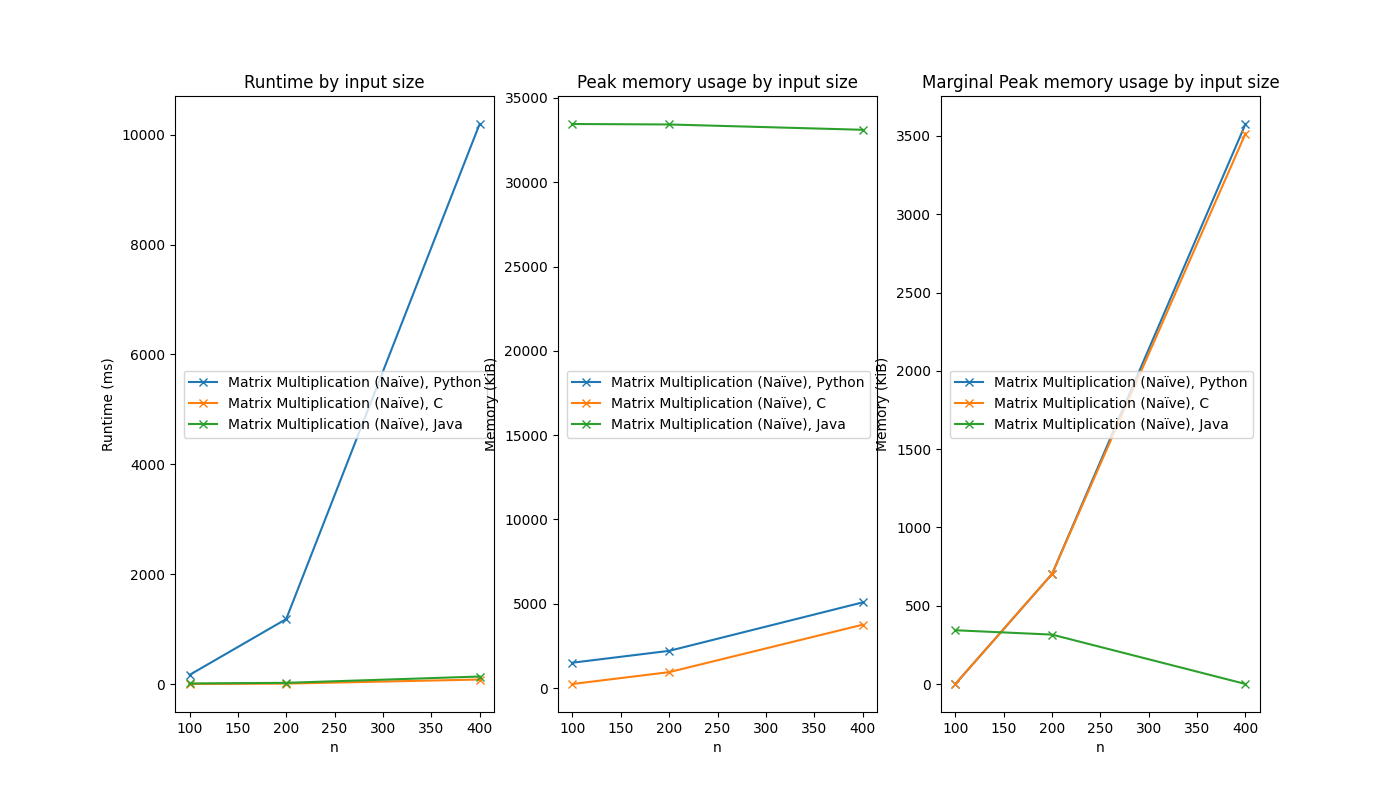
\includegraphics[width=\textwidth]{./matmul_naïve-plot.png}
  \caption{Performance of cannonical matrix multiplication.}
  \label{plot-matmul-cannonical}
\end{figure}

Figure~\ref{plot-matmul-cannonical} shows the performance of cannoncical matrix
multiplication. The leftmost graph shows the runtime of the benchmark. This
\emph{only} measures the benchmark itself, not any setup or tear-down. In this
case, runtime includes multiplying two matrices, but not allocating the input
matrices and filling them with random data.

The center graph shows peak memory usage, measured using Valgrind. This
measurement includes the entire benchmark program, including both setup and
tear-down. This is because there is no good way in Valgrind to determine what
part of the program is running at any given time. The rightmost graph shows
\emph{marginal} memory usage, which is the peak memory usage minus the lowest
peak memory usage of that program and benchmark, for any input. It is intented
to show the memory associated with increased input size, without any constant
overhead.

C did very well in this benchmark. At all input sizes, it was both the fastest
and used the least memory.

Python did very poorly on speed, taking 10 times the runtime as C on larger
input sizes. It performed much better on memory. Although Python carried a
\SI{1}{\mega B} overhead, this overhead was constant. In marginal memory usage
Python was very slightly worse than C.

Java on the other hand performed very well in runtime, with runtimes only
doubling that of C on larger inputs. Java's limitation was in terms of memory,
with performance \emph{considerably} worse than Python or C. This memory usage
was an overhead. Java's marginal memory usage appears very good, but that is
probably due to random variance in the memory overhead making the marginal
memory usage an invalid measurement.

\subsection{Heap}\label{heap}

\begin{figure}[H]
  \centering
  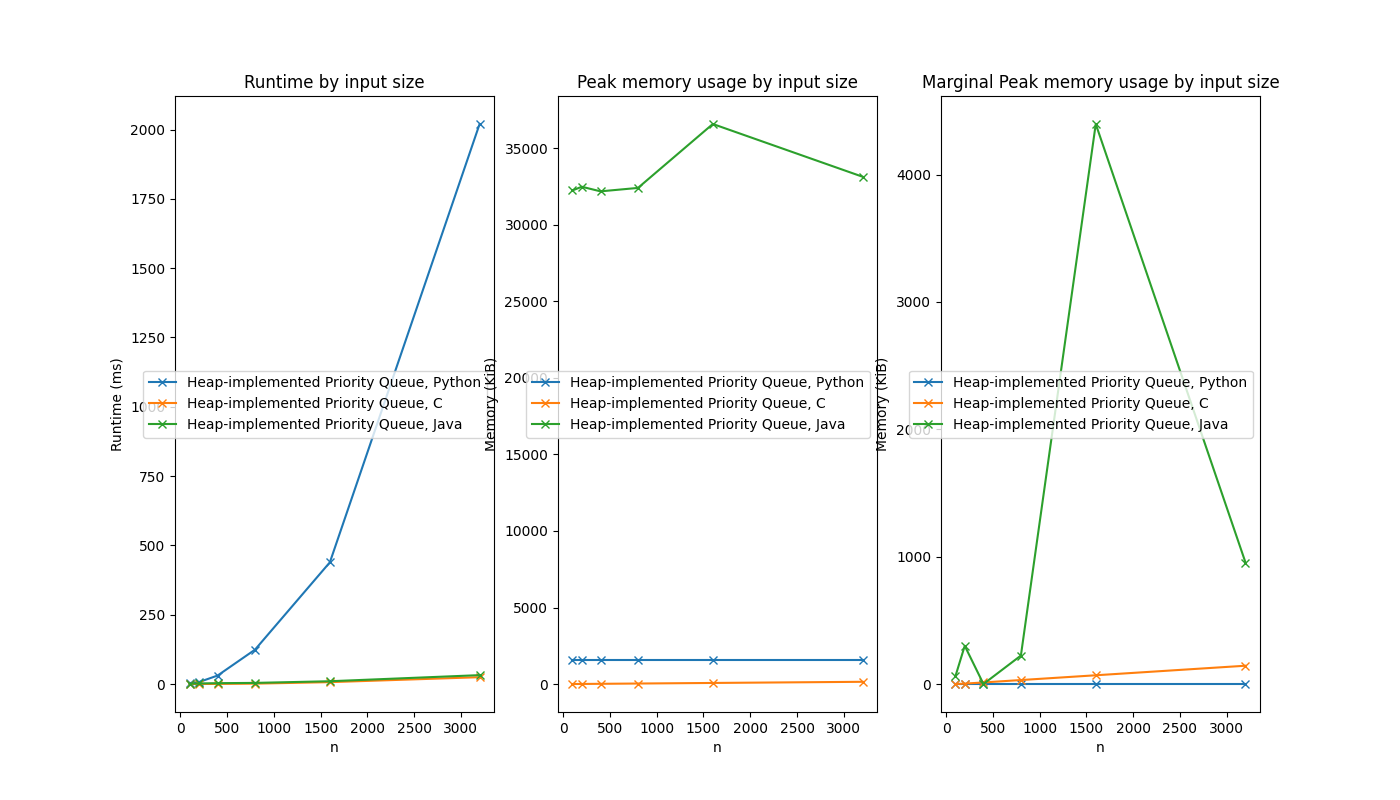
\includegraphics[width=\textwidth]{./heap-plot.png}
  \caption{Performance of a heap.}
  \label{plot-heap}
\end{figure}

Figure~\ref{plot-heap} shows the performance of my heap implementation. As
with~\ref{matmul-cannonical} Cannonical Matrix Multiplication, C's performance
was boring and efficient.

Python's performance was similar to~\ref{matmul-cannonical} Cannonical Matrix
Multiplication: memory was efficiency, constant overhead notwithstanding, but
runtime was very poor.

Java's performance\footnote{Java's results for this benchmark are different
that what I presented in class on April 22, 2022. I noticed a bug after the
presentation where the Java implementation skipped all the computation.} was
unremarkable. Like previously, it is roughly comparable to C.

\subsection{Standard Library Sorting}\label{sort}

\begin{figure}[H]
  \centering
  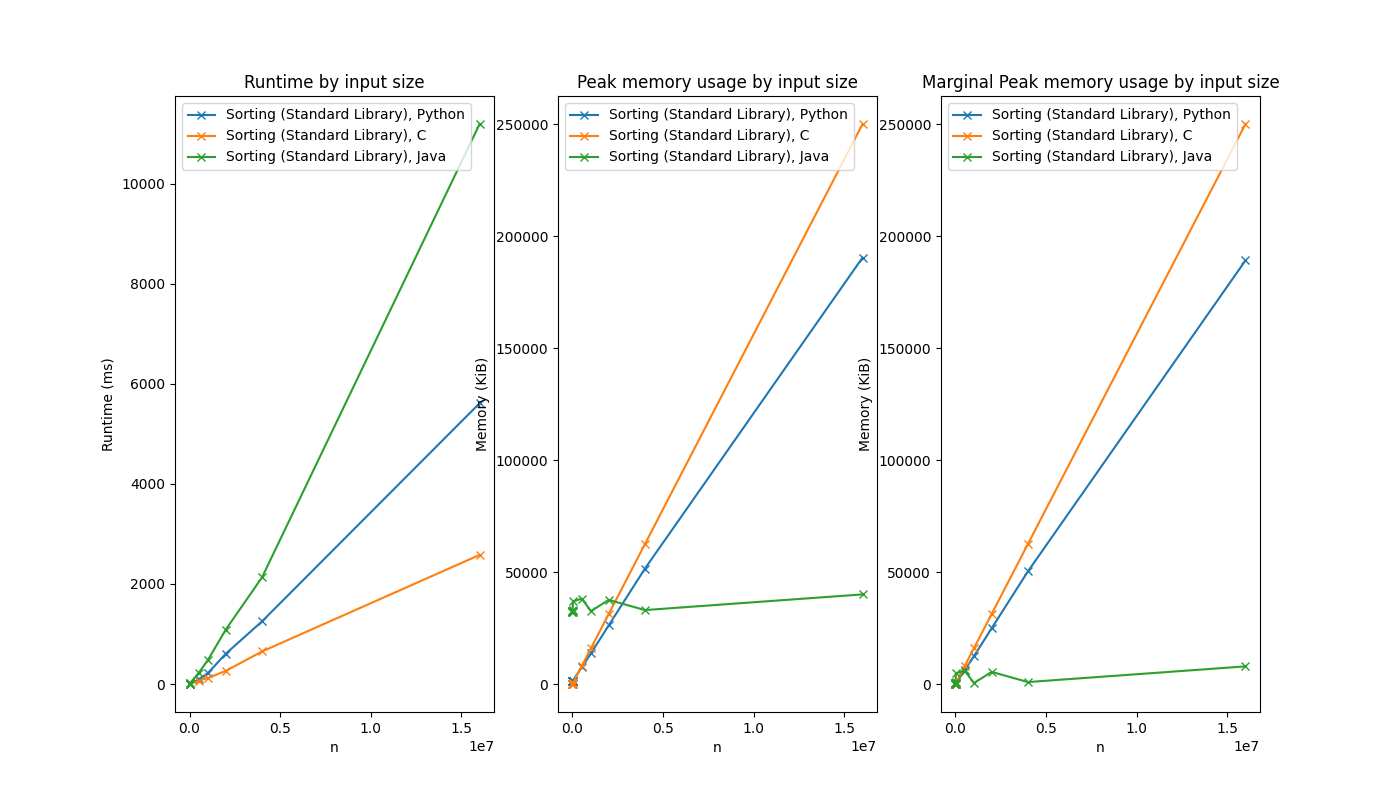
\includegraphics[width=\textwidth]{./sort_stdlib-plot.png}
  \caption{Performance of sorting via standard library functions.}
  \label{plot-sort}
\end{figure}

Figure~\ref{plot-sort} shows the performance of sorting via the various
language's standard library.  As usual, C was fast and efficient.

Python's performance on this benchmark was interesting. The runtime performance
was about double that of C. That doesn't seem impressive—it's still slower—but
in previous benchmarks it was orders of magnitude slower. As usual, Python's
memory performance was quite good. In fact, it was slightly better than C.
There are two main reasons for this: firstly, the memory requirements of
storing the input are high enough that the constant overhead is not noticable.
This is because Python's sort implementation is in-place\footnote{Per
\href{https://docs.python.org/3/library/stdtypes.html#list.sort}{Python's
documentation}.}, whereas C's implementation may not be in-place\footnote{In
the
\href{https://www.gnu.org/software/libc/manual/html_node/Array-Sort-Function.html}{GNU
specification}.} and thus require additional heap space.

Java's runtime performance was similar to how the language behaved previously:
worse than C, but not drastically so. It's memory performance on the other hand
was impossibly good, better than the theoretical minimum size of an array of
64-bit floats. This suggests that Valgrind may not accurately measure heap
memory in Java programs.

\subsection{Optimized Matrix Multiplication}\label{matmul-opt}

\begin{figure}[H]
  \centering
  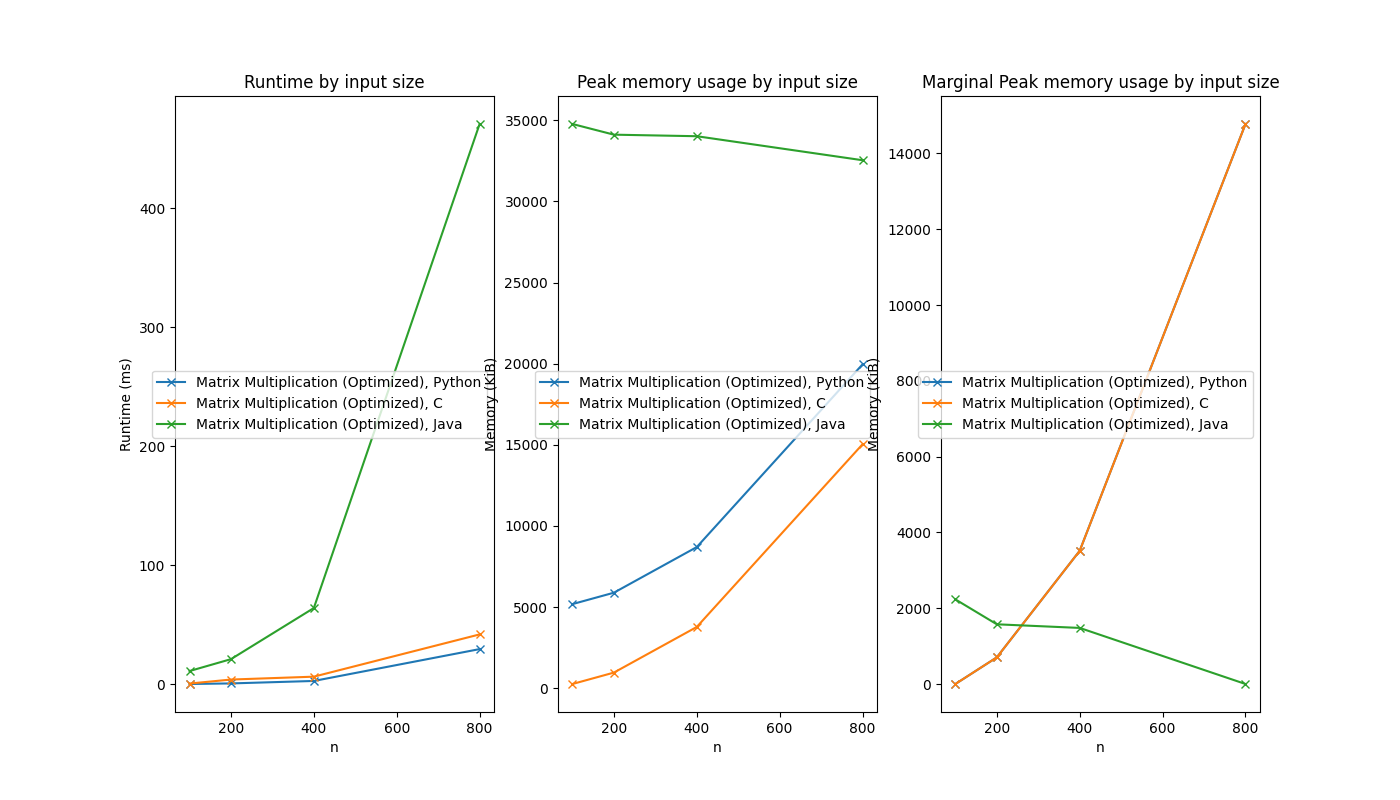
\includegraphics[width=\textwidth]{./matmul_optimized-plot.png}
  \caption{Performance of optimized matrix multiplication.}
  \label{plot-matmul-opt}
\end{figure}

Figure~\ref{plot-matmul-opt} shows the performance of sorting via
heavily-optimized third-party libries. This benchmark is intended to show what
the language can do when it is optimized to the greatest extend possible.

C's matrix multiplicaiton was done using the OpenBLAS\footnote{Basic Linear
Algebra System} library. As usual, C did reasonably well, but it was \emph{not}
the fastest in all cases.

Python used the popular Numpy library, although as discussed
in~\ref{numpy-blas}, this isn't \emph{quite} a correct statement. Impressively,
Python's performance at the largest input size was slightly better that C. It's
marginal memory performance was also very good, almost exactly equal to that of
C\footnote{This is why the Python line isn't visible on the marginal memory
usage graph: The Python line is exactly underneath the C line.}.

Java used the EJML linear algebra library. It's performance was unimpressive,
with runtimes larger than C, but within the same order of magnitude.

\section{Analysis}

\subsection{Why Python is so Slow}\label{python-slow}

Something that's very clear from~\ref{heap} Heap and~\ref{matmul-cannonical}
Cannonical Matrix Multiplication is that Python code is really, \emph{really}
slow.

On a high level, the reasons for this are rather simple. Firstly, C and Java
are both ahead-of-time compiled languages: transformantion of textual code to
computer-friently bytecode is done before runtime by a compiler, either GCC or
the Java Compiler. Python, on the other hand, is a JIT langauge, or
just-in-time compiled. Compilation is done \emph{at} runtime. This adds a time
overhead.

Python is also an interpreted language. C's bytecode is run directly on the
CPU's hardware, with no layer of indirection.\footnote{Except for the
indirection built into CPU itself, but that is common to all programs.} But
Python runs in the Python Interpreter, a program that interprets and runs your
code for you. Need to reference a variable? Your code has to ask the
interpreter to do it for you. Want to call a function? Again, the interpret
adds a (slow) layer in between your code and a function call on the CPU. All
this adds up to a significant slowdown.

Python isn't the only interpreted language in my sample: Java is also
interpreted: it runs in the Java Virtual Machine (JVM). But the JVM is more
efficient than the Python Interpreter, probably because it's a thinner
abstraction.

\subsection{Java Memory Overhead}

It's very apparent from all benchmarks that before allocating \emph{any}
significant data, Java has a large memory overhead, consistently
about~\SI{30}{\mega B}. This is because of the JVM. As it turns out, the JVM
has to store a lot of data about the code itself: compiled classes, field names
and function signatures, as well as the garbage collector. In particular,
compressed class space grows proportionally to the number of classes
loaded\footnote{Which in turn is roughly proportional to the complexity of your
code.}, and can easily dwarf the heap.

For more information, see
\href{https://spring.io/blog/2019/03/11/memory-footprint-of-the-jvm}{Memory
footprint of the JVM}, an article by Spring Blog that delves into this topic in
some detail. For my purposes, the main takeaway is that every Java process that
gets launched will immediatly take up \SI{30}{\mega B} of RAM.

The question I'm more interested in is this: is this a significant loss of
available memory? Well, it depends. Certainly it's problematic in embedded
applications where available memory is sometimes measured in bytes. But Java is
not commonly used for embedded tasks. Java is normally run on modern machines
like telephones and computers, where gigabytes of memory are available. Suppose
an application is being developed that will run on a server with \SI{128}{\giga
B} of ram available. Is this \SI{30}{\mega B} overhead significant? Again, it
depends. If the deployment plan is to run a handful of processes that each do
a lot of work, the memory overhead probably isn't significant. If the plan is
to run microservices, with thousands of process each doing a tiny piece of
work, then this tiny overhead is now taking up gigabytes of memory, and that
probably \emph{is} a problem.

\subsection{Why Sorting in Python \emph{isn't} Terrible}

As noted in~\ref{python-slow}, Python is rather painfully slow. Except,
in~\ref{sort} Sorting\footnote{It also wasn't slow in~\ref{matmul-opt}. I'll
address this in~\ref{numpy-blas}.}, it isn't. Why? Because the sorting isn't done
in Python code. It's done directly by the Python Interpreter. Or, to be more
precise, it's done by the CPython interpreter, since CPython is the Python
implementation under test. CPython is implemented in C. So Python's sorting is
implemented in C\footnote{For reference, see
\href{https://github.com/python/cpython/blob/f348154c8f8a9c254503306c59d6779d4d09b3a9/Include/listobject.h#L39}{the
header sorting where sorting is declared} and
\href{https://github.com/python/cpython/blob/f348154c8f8a9c254503306c59d6779d4d09b3a9/Objects/listobject.c#L2567-L2579}{the
implementation}.}\footnote{Presumably, if I tested Jython, it would be
implemented in Java.} which, as this project has made abaundantly clear, is
quite fast.

So speaking generally, what are the implications of this? It means that
although Python code runs slowly, standard library functions run quite quickly.
So will a performance-intensive application run in a reasonable time in Python?
It depends. If most of the computation happens within a standard library
function, it might run quite quickly.

\subsection{Why Python's Numpy is Fast}\label{numpy-blas}

So far, we've established that Python code is very slow, but Python standard
library functions can be fast, though not \emph{as} fast as C. So one would
expect that Python's optimized matrix multiplication runs very slowly. It's
certainly not a standard library function. And yet, Numpy's performance was
approximately the same as C, both in terms of runtime and in terms of marginal
memory usage.

How is this possible? Well, Python (or, at least, the popular CPython
implementation) has a rarely-used but enormously powerful feature: it can
interface nicely with C and C++
code\footnote{\href{https://docs.python.org/3/extending/extending.html}{Extending
Python with C or C++}}. This means that a Python program with a
performance-intensive component can implement that component in C, taking
advantage of C's efficiency. This is exactly how Numpy implements matrix
multiplication: in C. In fact, it uses OpenBLAS. Most of the work in the Python
matrix multiplication benchmark happens in a call to \texttt{cblas\_dgemm}, the
exact same function used in my C benchmark. So of \emph{course} Python's
performance was similar to C's: on some level, it was running exactly the same
code.

\clearpage
\section{Conclusion}\label{conclusion}

Before starting this project, I had a vague idea that C was very efficient and
Python was very slow, with most languages in the middle. In other words, to
program in a easy-to-use language like Python, you have to pay the price of
worse performance. My goal in this project was to quantify this cost, with the
ultimate goal of helping answer the question of whether that cost is worth it.

To absolutely no one's surprise, the answer is that \emph{it depends}.

The performance penalty will depend not only on what language is used, but also
on \emph{how} that language is used. Python is the most extreme example of
this. A pure-Python implementation might be very slow. But what if an
application is \SI{90}{\%} Python, \SI{10}{\%} C? If the performance-intensive
part is in C, you can sort of get the best of both worlds: most of your code is
built in the easy-to-use Python, but code that has to run fast is built in the
more efficient C.

Ultimately, every language will have advantages and disadvantages. To
intelligently choose the best language for a particular task, one needs to know
what these advantages and disadvantages are. To that end, here are listed the
specific, objective results of this project:

\begin{itemize}
  \item The runtime of Python code can be over 100 times the runtime of
    equivalent C code.
  \item The runtime of Java code is generally about double the runtime of
    equivalent C code.
  \item Each Python process introduces a memory overhead of approximately
    \SI{100}{\kilo B}.
  \item Each Java process introduces a memory overhead of approximately
    \SI{30}{\mega B}.
  \item The memory overhead of loading a small C program is negligible for
    most purposes.
  \item The marginal cost of allocating more data in Python is not materially
    different than allocating equivalent data in C.
  \item The marginal cost of allocating more data in Java is difficult to
    measure.
  \item Python standard library functions can be nearly as fast or as fast as
    their C equivalents. The same is true of third-party libraries that have
    implemented some of their functionality in C.
  \item CPython allows easy integration with C code, meaning that a Python
    codebase can, in some cases, be easily accelerated by implementing a small
    portion of the codebase in C.
\end{itemize}

\appendix

\section{Computer Specifications}

These benchmarks can be run on any AMD-64 computer. Since runtimes are only
compared to each other, running on different computers shouldn't meaningfully
affect results. Additionally, since all benchmarks are single-threaded, the
number of available cores shouldn't affect performance.

However, the specifications of the test machine are listed below, collected
using Inxi via \texttt{inxi --admin --verbosity=7 --filter}.

\lstinputlisting[]{./specs.inxi}

\section{License}\label{license}

\lstinputlisting{./LICENSE}

\end{document}
